\chapter{
Introduction
}
\markboth{Introduction}{}
\label{chapt.intro}

\vspace{.3in}

Knowledge of the spatial structure of populations is central to
applied and theoretical population ecology, landscape ecology,
conservation biology and many other ecological disciplines.  For
example, understanding distribution and spatial variation in density
are important in the management of populations, and movement,
dispersal, and space usage are important to understanding landscape
connectivity.
%and density dependence, and spatial interactions among individuals
%contribute to these population processes.
At the same time, the inherent spatial aspect of {\it sampling}
populations strongly affects apparent biases in how we observe
population structure.

Many texts and more focused monographs have addressed the concepts and
relevance of spatial processes in animal populations
\citep{tilman_kareiva:1997,hanski:1999, clobert_etal:2001}. Similarly,
many synthetic treatments exist on techniques and models for sampling
populations using capture-recapture methods
\citep{seber:1982,borchers_etal:2002,williams_etal:2002,cooch_white:2006}.
However, despite the central roll of space and spatial processes to
both understanding population dynamics and how we observe or sample
populations, a coherent framework that integrates these two aspects of
ecological systems has not been fully realized either conceptually or
methodologically.

Capture-recapture methods represent perhaps the most common technique
for studying animal populations, and their use is growing in
popularity due to recent technological advances that expand their
utility to many taxa which before could not be studied efficiently, if
at all.  However, a major deficiency of classical capture-recapture
methods is that they do not admit the spatial structure of either
ecological processes that give rise to encounter history data, nor the
spatial aspect of collecting these data. While many technical
limitations of this lack of spatial explicitness have been recognized
for decades \citep{dice:1938, hayne:1950}, it has only been very
recently \citep{efford:2004,borchers:2011} that spatially explicit
capture-recapture methods -- those which accomodate space -- have been
developed.

Spatial capture-recapture (SCR) methods resolve a host of technical
problems that arise in applying capture-recapture methods to animal
populations.  However, SCR models are not merely an extension of
technique. Rather, they represent a much more profound extension in
that they make ecological processes explicit in the model -- processes
of density, spatial organization, movement and space-usage by
individuals.  The practical importance of SCR models is that they
allow ecological scientists to study elements of ecological theory
using observational data that exhibit various biases relating to the
observation mechanisms employed. In the context of capture-recapture,
we observe individual encounter history data from which, using SCR
models, we can infer where individual live, how they organize
themselves spatially and move around in space and how they interact
with other individuals.  Thus, SCR models enable ecologists to
explicitly integrate biological context and theory with encounter
history data, in order to address questions of population demography,
space usage, movement, environmental or landscape effects on density
and other processes, and other important elements of ecological
theory.
At the same time, SCR models can be
 used, and may be the only option, for obtaining baseline data on some of
 the rarest and most elusive species---information which is required
 for effective conservation.
 Their potential for advancing both
 applied and theoretical research has not been fully
 realized, which is one reason that compelled us to write this book.

\section{The Study of Populations by Capture-Recapture}

Information about abundance or density of populations, and their vital
rates, is fundamental to applied ecology and conservation biology.  To
that end, a huge variety of statistical methods have been devised, and
among these, the most well-developed are collectively known as
capture-recapture (or capture-mark-recapture) methods. For example,
the volumes by \citet{otis_etal:1978}, \citet{white_etal:1982},
\citet{seber:1982}, \citet{pollock_etal:1990},
\citet{borchers_etal:2002}, \citet{williams_etal:2002}, and
\citet{amstrup_etal:2005} are largely synthetic treatments of such
methods, and contributions on modeling and estimation using
capture-recapture are plentiful in the peer-reviewed ecology
literature.
%Capture-recapture techniques have been the number 1 quantiative method
%in studies of animal populations for decades.
%But they apply basically to fish bowl sampling. Does it make sense
%that methods should apply to both?

Capture-recapture techniques make use of individual {\it encounter
  history} data, by which we mean sequences of (usually) 0's and 1's
denoting if an individual was encountered during sampling over a
certain time period. For example, the encounter history ``010''
indicates that this individual was encountered only during the second
of three trapping occasions. As we will see, these data contain
information about encounter probability, and also abundance, and other
parameters of interest in the study of populations.

Capture-recapture methods have been important in studies of animal
populations for many decades, and their importance is growing
dramatically in response to technological advances that improve our
ability and efficiency to obtain encounter history data. Historically,
such information was obtainable using methods requiring physical
capture of individuals.  However, new methods do not require physical
capture or handling of individuals.  A large number of passive
detection devices produce individual encounter history data including
camera traps \citep{karanth_nichols:1998, oconnell_etal:2010},
acoustic recording devices \citep{dawson_efford:2009}, and methods
that obtain DNA samples such as hair snares for bears, scent posts for
many carnivores, and related methods which allow DNA to be extracted
from scat, urine or animal tissue in order to identify individuals.
This book is concerned with how such data can be used to carry out
inference about animal abundance or density, and other parameters such
as survival, recruitment, resource selection, and movement using new
classes of capture-recapture models which utilize auxiliary spatial
information related to the encounter process.  We refer to such
methods as spatial capture-recapture (SCR) models\footnote{In the
  literature the term spatially explicit capture-recapture (SECR) is
  also used, but we prefer the more concise term.}.

As the name implies, the primary feature of SCR models that
distinguishes them from traditional CR methods is that they make use
of the spatial information inherent to capture-recapture studies.
Encounter histories that are associated with auxiliary information on
the location of capture, are {\it spatial encounter histories}. This
auxiliary information is informative about spatial processes including
the spatial organization of individuals, variation in density,
resource selection and space usage, and movement.  As we will see, SCR
models allow us to overcome critical deficiencies of non-spatial
methods, and integrate ecological theory with encounter history
data. As a result, this greatly expands the practical utility and
scientific relevance of capture-recapture methods, and studies that
produce encounter history data.

% to use capture-recapture data in the form of encounter history data
% to study explicit ecological hypotheses about spatial variation and
% space usage.  namely, traditional CR methods cannot be used to
% formally estimate density, include of trap-level covariates of
% density or capture probability, or account for heterogeneity in
% encounter probability that results from the spatial organization of
% animals and traps.  Thus, spatial modeling is not just a fun
% academic exercise; it provides a solution to basic problems in the
% study of animal populations that have been acknowledged for more
% than 70 years \citep{dice:1938}.  More important than just providing
% a resolution to some basic technical problems, SCR models provide a
% framework for
%%integrate into capture-recapture models explicit ecological hypotheses
%%related to spatial population processes.  In turn, this greatly
%%expands the practical utility and scientific relevance of
%%capture-recapture methods and studies based on encounter history data.

\section{Lions and Tigers and Bears, oh my:
Genesis of Spatial capture-recapture data}

A diverse number of methods and devices exist for producing individual
encounter history data with auxiliary spatial information about
individual locations. Historically, physical ``traps'' have been
widely used to sample animal populations. These include live traps,
mist nets, pitfall traps and many other types of devices. Such devices
physically retain animals until visited by a biologist, who removes
the individual, marks it or otherwise molests it in some scientific
fashion, and then releases it.  Although these are still widely used,
recent technological advances for obtaining encounter history data
non-invasively have made it possible to study many species that were
difficult if not impossible to study effectively just a few years ago.
As a result, these methods have revolutionized the study of animal
populations by capture-recapture methods, have inspired the
development of spatially-explicit extensions of capture-recapture, and
will lead to their increasing relevance in the future.  We briefly
review some of these here, which we consider more explicitly in later
chapters of this book.

\subsection{Camera trapping}

Considerable recent work has gone into the development of
camera-trapping methodologies. For a historical overview of this
method see \citet{kays_etal:2008} and \citet{kucera_barrett:2011}.
Several recent synthetic works have been published including
\citet{nichols_karanth:2002}, and an edited volume by
\citet{oconnell_etal:2010} devoted solely to camera trapping concepts
and methods. As a method for estimating abundance, some of the
earliest work that relates to the use of camera trapping data in
capture-recapture models originates from Karanth and colleagues
\citep{karanth:1995, karanth_nichols:1998, karanth_nichols:2000}.

\begin{figure}[ht]
\begin{center}
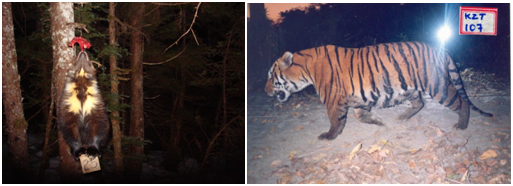
\includegraphics[width=5in]{Ch1/figs/wolverinetiger}
\end{center}
\caption{
Left: Wolverine being encounter by a
camera trap ({\it Photo credit: Audrey Magoun}).
Right: Tiger encountered by
camera trap ({\it Photo credit: Ullas Karanth}).
}
\label{fig.wolverinetiger}
\end{figure}

In camera trapping studies, cameras are situated along trails or at
baited stations and individual animals are photographed and
subsequently identified either manually by a person sitting behind a
computer, or sometimes now using specific identification
software. Camera trapping methods are widely used for species that
have unique stripe or spot patterns such as tigers
\citep{karanth:1995, karanth_nichols:1998}, ocelots ({\it Leopardus
  pardalis }; \citep{trolle_kery:2003,trolle_kery:2005}), leopards
({\it Panthera pardus}; \citep{balme_etal:2010}), and many other cat
species.  Camera traps are also used for other species such as
wolverines ({\it Gulo gulo};
\citep{magoun_etal:2011,royle_etal:2011jwm}), and even species that
are less easy to identify uniquely such as mountain lions ({\it Puma
  concolor}, \citep{sollmann_etal:inprepjapplecol}) and coyotes ({\it
  Canis latrans}, \citep{kelly_etal:2008}).  We note that even for
species that are not readily identified by pelage patterns, it might
be efficient to use camera traps in conjunction with spatial
capture-recapture models to estimate density (see
Chapts.~\ref{chapt.scr-unmarked} and \ref{chapt.partialID}).
%, if an initial sample of individuals can be collared
%or tagged in some way so that subsequent encounter by camera-traps can
%yield individual information. In this way, the probability of
%encounter can be estimated from the camera traps based on the
%pre-marked individuals, and this is applied to the frequencies of
%unmarked individuals to estimate density.







\subsection{DNA sampling}

DNA obtained from hair, blood or scat is now routinely used to obtain
individual identity and encounter history information about
individuals \citep{taberlet_bouvent:1992, kohn_etal:1999,
  woods_etal:1999, mills_etal:2000, schwartz_monfort:2008}.  A common
method is based on the use of ``hair snares'' (Fig. \ref{fig.bearcat})
which are widely used to study bear populations
\citep{woods_etal:1999, gardner_etal:2010jwm, garshelis_etal:2006,
  kendall_etal:2009}.  A sample of hair is obtained as individuals
pass under or around barbed-wire (or other physical mechanism) to take
bait. Hair snares and scent sticks have also been used to sample felid
populations \citep{garciaalaniz_etal:2010, kery_etal:2010} and other
species. Research has even shown that DNA information can be extracted
from urine deposited in the wild (e.g., in snow; see
\cite{valiere_taberlet:2000}) and as a result this may prove another
future data collection technique where SCR models are useful.

\begin{figure}
\begin{center}
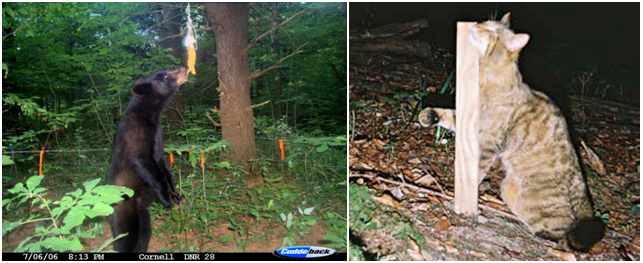
\includegraphics[width=5in]{Ch1/figs/bearcat}
\end{center}
\caption{Left:  Black bear in a hair snare ({\it Photo credit: M. Wegan})
Right: European wildcat loving on a scent stick ({\it Photo credit: Darius
Weber
%, Hintermann \& Weber AG, Ecological Consultancy, Planning \&
%Research, Switzerland
})
}
\label{fig.bearcat}
\end{figure}


\begin{figure}
\begin{center}
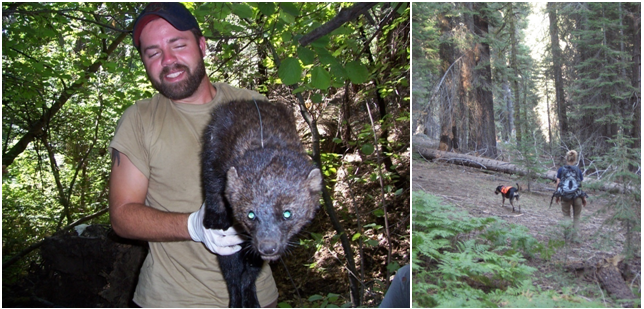
\includegraphics[width=5in]{Ch1/figs/beardog}
\end{center}
\caption{Left:
A wildlife research technician for the USDA Forest Service
  holding a male fisher  captured as part of the Kings River Fisher
  Project in the Sierra National Forest, California.
Right: A dog handler surveying for fisher scat in the Sierra National Forest.
{\it Photo credit: Craig Thompson}.}
%, USDA Forest Service,
%Pacific Southwest Research Station.}}
\label{fig.fisherscatdog}
\end{figure}


\subsection{Acoustic sampling}

Many studies of birds \citep{dawson_efford:2009}, bats, and whales
\citep{marques_etal:2009} now collect data using devices that record
vocalizations. When vocalizations can be identified by individual from
multiple recording devices, spatial encounter histories are produced
that are amenable to the application of SCR models
\citep{dawson_efford:2009, efford_etal:2009ecol}. Recently, these
ideas have been applied to data on direction  or distance to
vocalizations by multiple simultaneous observers and related problems
(D. Borchers, ISEC 2012 presentation).


\subsection{Search-encounter methods}

There are other methods which don't fall into a nice clean taxonomy of
``devices''. Spatial encounter histories are commonly obtained by
conducting manual searches of geographic sample units such as
quadrats, transects or road or trail networks.  For example, DNA-based
encounter histories can be obtained from scat samples located along
roads or trails or by specially trained dogs \citep{mackay_etal:2008}
searching space (Fig. \ref{fig.fisherscatdog}). This method has been
used in studies of martens, fishers \citep{thompson_etal:2012},
lynx, coyotes, birds \citep{kery_etal:2010}, and many other species.
A similar data structure arises from the use of standard territory or
spot mapping of birds \cite{bibby_etal:1992} or area sampling in which
space is searched by observers to physically capture individuals.
This is common in surveys that involve reptiles and amphibians, e.g.,
we might walk transects picking up box turtles \citep{hall_etal:1999},
or desert tortoises \citep{zylstra_etal:2010}, or search space for
lizards \citep{royle_young:2008}.

These methods don't seem like normal capture-recapture in the sense
that the encounter of individuals is not associated with specific trap
location, but SCR models are equally relevant for analysis of such
data as we discuss in Chapt. \ref{chapt.search-encounter}.




\section{Capture-Recapture for Modeling Encounter Probability}

We briefly introduced techniques used for the study of animal
populations. These methods produce individual encounter history data,
a record of where and when each individual was captured. We refer to
this as a {\it spatial encounter history}. Historically, auxiliary
spatial information has been ignored, and encounter history data have
been {\it summarized} to simple ``encounter or not'' for the purpose
of applying ordinary CR models.  The basic problem with these ordinary
(or ``non-spatial'') capture-recapture models is they don't have any
sense of space in them, the spatial information is summarized out of
the data set, so we aren't able to use such models for studying things
such as movement, or resource selection, etc..  Instead, ordinary
capture-recapture models usually resort to models of ``encounter
probability,'' which is a nuisance parameter, seldom of any ecological
relevance.  We show an example here that is in keeping with the
classical application of ordinary capture-recapture models.

%In terms of density estimation,  there is no
%linkage {\it in the model} between the quantity being informed by the
%data (i.e., $N$) and any stated or prescribed ``area'', $A$.



\subsection{Example: Fort Drum bear study}

Here we confront the simplest possible capture-recapture problem,
estimating density from a standard capture-recapture study, but one of
some applied interest. We use this as a way to introduce some concepts
and motivate the need for spatial capture-recapture models by
confronting technical and conceptual problems that we encounter. The
data come from a study to estimate black bear abundance on the Fort
Drum Military Installation in upstate New York (see
Chapt. \ref{chapt.closed} for more details). The specific data used
here are encounter histories on 47 individuals obtained from an array
of 38 baited ``hair snares'' during June and July 2006. The study area
and locations of the 38 hair snares are shown in
Fig. \ref{fig.hairsnares}.  Barbed wire traps (see
Fig. \ref{fig.bearcat}) were baited and checked for hair samples each
week for eight weeks.  Analysis of these data appears in
\citet{gardner_etal:2010jwm} and we use the data in a number of
analyses in later chapters.

\begin{figure}[ht]
\begin{center}
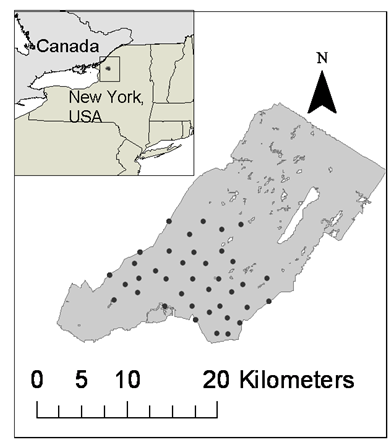
\includegraphics[height=3in]{Ch1/figs/hairsnares}
\end{center}
\caption{Locations of hair snares on Fort Drum, New York, operated
  during the summer of 2006 to sample black bears.}
\label{fig.hairsnares}
\end{figure}

Although each bear was captured, or not, in each of the 38 hair
snares, we treat this data set as a standard capture-recapture data
set and summarize to an encounter history matrix with 47 rows and 8
columns with entries $y_{ik}$, where $y_{ik}=1$ if individual $i$ was
captured, at any trap, in sample occasion $k$ and $y_{ik}=0$
otherwise. There is a standard closed population model, colloquially
referred to as ``model $M_0$'' (see Chapt. \ref{chapt.closed}), which
assumes that encounter probability $p$ is constant for all individuals
and sample periods.  We fitted model $M_0$ to the Fort Drum data using
traditional likelihood methods, yielding the maximum likelihood
estimate (MLE) of $\hat{N} = 49.19$ with an asymptotic standard error
(SE) of $1.9$.

The key issue in using such a closed population model regards how we
should interpret this estimate of $N=49.19$ bears. Does it represent
the entire population of Fort Drum? Certainly not -- the trapping
array covers less than half of Fort Drum as we see in
Fig. \ref{fig.hairsnares}. So to get at the total bear population size
of Fort Drum, we would have to convert our $\hat{N}$ to an estimate of
density and extrapolate. To get at density, then, should we assert
that $N$ applies to the southern half of Fort Drum below some
arbitrary line? Surely bears move on and off of Fort Drum without
regard to hypothetical boundaries. Without additional information
there is simply no way of converting this estimate of $N$ to density,
and hence it is really not meaningful biologically. To resolve this
problem, we will adopt the customary approach of converting $N$ to $D$
by buffering the convex hull around the trap array. The convex hull
has area $157.135$ $km^2$. We follow \citet{bales_etal:2005} in
buffering the convex hull of the trap array by the radius of the mean
female home range size.


%%%%\footnote{Did Bales et al. actually do this?}.
%HERE IS WHAT BALES DID:  First, we created a 95% minimum convex polygon
%for all radiolocations of adult females used in homerange
%analyses (Figure 1). Second,we buffered the
%100% minimum convex polygon for trapping locations
%with the approximate radius of the average
%95% minimum convex polygon home range of adult
%females (n = 13) using ArcView (ESRI, Redlands,
%Calif.).

The mean female home range radius was estimated \citep{wegan:2008} for
our study region to be $2.19$ km,
%\footnote{Is this number right out of Wegan's disseration?}
% YES, this is straight out of his thesis.
and the area of the convex hull buffered by $2.19$ km is $277.01$
km$^2$. ({\bf R} commands to compute the convex hull, buffer it, and
compute the area are given in the {\bf R} package \mbox{\tt scrbook}
which accompanies the book).  Hence, the estimated density here is
approximately $0.178$ bears/km$^2$ using the estimated population size
obtained by model $M_0$.  We could assert that the problem has been
solved, go home, and have a beer.  But then, on the other hand, maybe
we should question the use of the estimated home range radius -- after
all, this is only the female home range radius and the home ranges
change for many reasons. Instead, we may decide to rely on a buffer
width based on one-half mean maximum distance moved (MMDM) estimated
from the actual hair snare data as is more customary
\citep{dice:1938}. In that case the buffer width is $1.19$ km, and the
resulting estimated density is increased to $0.225$ bears/km$^2$ about
27 \% larger.  But wait -- some studies actually found the full MMDM
\citep{parmenter_etal:2003} to be a more appropriate measure of
movement (e.g \citet{soisalo_cavalcanti:2006}). So maybe we should use
the full MMDM which is $2.37$ km, pretty close to the telemetry-based
estimate and therefore providing a similar estimate of density
($0.171$ bears/km$^2$). So in trying to decide how to buffer our trap
array we have already generated 3 density estimates. The crux of the
matter is obvious: Although it is intuitive that $N$ should scale with
area -- the number of bears should go up as area increases and go down
as area decreases -- in this ad hoc approach of accounting for animal
movement $N$ remains the same, no matter what area we assert was
sampled. The number of bears and the area they live in are not
formally tied together within the model, because estimating $N$ and
estimating the area $N$ relates to are two completely independent
analytical steps which are unrelated to one another by a formal model.

Unfortunately, our problems don't end here. In thinking about the use
of model $M_0$, we might naturally question some of the basic
assumptions that go into that model. The obvious one to question is
that which declares that $p$ is constant. One obvious source of
variation in $p$ is variation {\it among individuals}. We expect that
individuals may have more or less exposure to trapping due to their
location relative to traps, and so we try to model this
``heterogeneous'' encounter probability phenomenon.
To illustrate
this phenomenon,  here are the
number of traps that each individual
was encountered in:
\begin{verbatim}
 # traps:  1   2  3  4  5  6  9
 # bears: 23  13  6  2  1  1  1
\end{verbatim}
meaning, for example, 23 bears were captured in only 1 trap, and 1
bear was captured in 9 distinct traps. The variation in trap-encounter
frequencies suggests quite a range in traps exposed to bears in the
sampled population.
%%% #bears: 19 15  5  2  2  1  1  1  1
% But, being captured in different numbers of traps is {\it not}
% inconsistent with a non-spatial model.  That is if individuals
% roamed randomly over space with no ``home range'' then you should
% expect them to be captured in varying numbers of traps also.....
Historically, researches try to reduce spatial heterogeneity in
capture probability by placing $>1$ trap per home range
\citep{otis_etal:1978, williams_etal:2002}. This seems like a sensible
idea but it is difficult to do in practice since you don't know where
all the home ranges are and so we try to impose a density of traps
that averages something $>1$ per home range.  An alternative solution
is to fit models that allow for individual heterogeneity in $p$
\citep{karanth:1995}. Such models have the colloquial name of ``model
$M_h$'' \citep{otis_etal:1978}.  We fitted this model (see
Chapt. \ref{chapt.closed} for details) to the Fort Drum data using
each of the 3 buffer widths previously described (telemetry, 1/2 MMDM
and MMDM), producing the estimates reported in Table
\ref{intro.tab.fdests}. While we can tell by the models' AIC that
$M_h$ is clearly favored by more than 30 units, we might still not be
entirely happy with our results. Clearly there is information in our
data that could tell us something about the exposure of individual
bears to the trap array -- where they were captured, and how many
times -- but since space has no representation in our model, we can't
make use of this information. Model $M_h$ thus merely accounts for
what we observe in our data (some bears were more frequently captured
than others) rather than explicitly accounting for the processes that
generated the data.

So what are we left with?  Our density estimates span a range from
$0.17$ to $0.43$ bears/km$^2$ depending on which estimator of $N$ we
use and what buffer strip we apply. Should we feel strongly about one
or the other?  Which buffer should we prefer?  AIC favors model $M_h$,
but did it adequately account for the differences in exposure of
individuals to the trap array? Are we happy with a purely
phenomenological model for heterogeneity?  It assumes that all
individuals are independent and identically distributed ($iid$) draws
from some distribution, but does not account for the explicit
mechanism of induced heterogeneity. And, further, we have information
about that (trap of capture) which model $M_h$ ignores.
% Moreover, we could find more variations of model Mh to choose among,
% but see \citep{link:2003}.
And if we choose one type of buffer, how do we compare our density
estimates to those from other studies that may opt for a different
kind of buffer?  The fact that $N$ does not scale with $A$, as part of
the model, renders this choice arbitrary.



\begin{table}[ht]
\centering
\caption{Table on estimates of density ($D$, bears/$km^2$) for the Fort Drum data
using models $M_0$ and $M_h$ and different buffers. Model $M_h$ here
is a logit-normal mixture \citep{coull_agresti:1999}.}
\begin{tabular}{ll|cc}
\hline \hline
Model & Buffer &  $\hat{D}$ & SE \\ \hline
$M_0$   & telemetry &  0.178 & 0.178 \\
$M_0$    & MMDM     &  0.171 & 0.171\\
$M_0$   & 1/2 MMDM  &  0.225 & 0.225\\
$M_h$ & telemetry &0.341 & 0.144\\
$M_h$ & MMDM    &  0.327 & 0.138\\
$M_h$ & 1/2 MMDM & 0.432 & 0.183\\ \hline
\end{tabular}
\label{intro.tab.fdests}
\end{table}


\subsection{Inadequacy of non-spatial capture-recapture}

The parameter $N$ (population size) in an ordinary capture-recapture
model is functionally unrelated to any notion of sample area, and so
we are left taking arbitrary guesses at area, and matching it up with
estimates of $N$ from different models that do not have any explicit
biological relevance.  Clearly, there is not a compelling solution to
be derived from this ``estimate $N$ and conjure up a buffer'' approach
and we are left not much wiser about bear density at Fort Drum than we
were before we conducted this analysis, and certainly not confident in
our assessments.  Closed population models are not integrated with any
ecological theory, so our $N$ is not connected to the specific
landscape in any explicit way.

The capture-recapture models that we used apply to truly closed
populations -- a population of goldfish in a fish bowl. Yet here we
are applying them to a population of bears that inhabit a rich
two-dimensional landscape of varied habitats, exposed to trapping by
an irregular and sparse array of traps. It seems questionable that the
same model that is completely sensible for a population of goldfish in
a bowl, should also be the right model for this population of bears
distributed over a broad landscape.  Ordinary capture-recapture
methods are distinctly non-spatial. They don't admit spatial indexing
of either sampling (the observation process) or of individuals (the
ecological process). This leads immediately to a number of practical
deficiencies: (1) Ordinary CR models do not provide a coherent basis
for estimating density, a problem we struggled with in the black bear
study.  (2) Ordinary CR model and sampling methods {\it induce} a form
of heterogeneity that can only at best be approximated by classical
models of latent heterogeneity. SCR models formally accommodate
heterogeneity due to the juxtaposition of individuals with the
encounter devices.  (3) Ordinary CR models do not accommodate
trap-level covariates which exist in a large proportion of real
studies; (4) Ordinary CR models do not accommodate formal
consideration of any spatial process that gives rise to the observed
data.

In subsequent chapters of this book, we resolve these specific
technical problems related to density, model-based linkage of N and A,
covariates, spatial variation, and related things all within a
coherent unified framework for spatial capture-recapture.


\section{ Historical Context: A Brief Synopsis}

Spatial capture-recapture is a relatively new methodological
development, at least with regard to formal estimation and
inference. However, the basic problems that motivate the need for
formal spatially-explicit models have been recognized for decades and
quite a large number of ideas have been proposed to deal with these
problems. We review some of these ideas here.

\subsection{Buffering}

The standard approach to estimating density even now is to estimate
$N$ using conventional closed population models \citep{otis_etal:1978}
and then try to associate with this estimate some specific sampled
area, say $A$, the area which is contributing individuals to the
population for which $N$ is being estimated. The strategy is to define
$A$ by placing a buffer of say $W$ around the trap array or some
polygon which encloses the trap array. The historical context is
succinctly stated by \citep{obrien:2011} from which we draw this
description:

\begin{quote}
  ``At its most simplistic, $A$ may be described by a concave polygon
  defined by connecting the outermost trap locations ($A_{tp}$;
  \citet{mohr:1947}).  This assumes that animals do not move from
  outside the bounded area to inside the area or vice versa. Unless
  the study is conducted on a small island or a physical barrier is
  erected in the study area to limit movement of animals, this
  assumption is unlikely to be true. More often, a boundary area of
  width $W$ ($A_{w}$) is added to the area defined by the polygon
  $A_{tp}$ to reflect the area beyond the limit of the traps that
  potentially is contributing animals to the abundance estimate
  \citep{otis_etal:1978}. The sampled area, also known as the
  effective area, is then $A(W) = A_{tp} + A_{w}$. Calculation of the
  buffer strip width ($W$) is critical to the estimation of density
  and is problematic because there is no agreed upon method of
  estimating $W$. Solutions to this problem all involve ad hoc methods
  that date back to early attempts to estimate abundance and home
  ranges based on trapping grids
  \citep[see][]{hayne:1949}. \citet{dice:1938} first drew attention to
  this problem in small mammal studies and recommended using one-half
  the diameter of an average home range. Other solutions have included
  use of inter-trap distances \citep{blair:1940, burt:1943}, mean
  movements among traps, maximum movements among traps
  \citep{holdenried:1940, hayne:1949}, nested grids
  \citep{otis_etal:1978}, and assessment lines
  \citep{smith_etal:1971}.''
\end{quote}

The idea of using 1/2 mean maximum distance moved
\citep[``MMDM''][]{wilson_anderson:1985a} to create a buffer strip
seems to be the standard approach even today, presumably justified by
Dice's suggestion to use 1/2 the home range diameter, with the mean
over individuals of the maximum distance moved being an estimator of
home range diameter. Alternatively, some studies have used the full
MMDM (e.g. \citet{parmenter_etal:2003}), because the trap array might
not provide a full coverage of the home range (home ranges near the
edge should be truncated) and so 1/2 MMDM should be biased smaller
than the home range radius.  And, sometimes home range size is
estimated by telemetry \citep{karanth:1995, bales_etal:2005}.
% \footnote{Is this correct cite for this?}.  Karanth used some
% technique, it's hard to tell for sure....but he mentions using 1
% female that is collared to estimate effective trap area.  Bales does
% it too, so I added it for extra value!
Use of MMDM summaries to estimate home range radius is usually
combined with an AIC-based selection from among the closed-population
models in \citet{otis_etal:1978} which most often suggests
heterogeneity in detection (model $M_h$).  Almost all of these early
methods were motivated by studies of small mammals using classical
``trapping grids'' but, more recently, their popularity in the study
of wildlife populations has increased with the advent of new
technologies, especially related to non-invasive sampling methods such
as camera trapping. In particular, the series of papers by Karanth and
Nichols \citep{karanth:1995, karanth_nichols:1998,
  karanth_nichols:2002} has led to fairly widespread adoption of these
ideas.

\begin{comment}
Some of the heuristic ideas based on buffer strips do have some
technical justification in the sense of estimating parameters of an
underlying movement model from observed movements. For example, if we
let $x$ be a random variable indicating movement outcomes of an
individual about its  home range center, and suppose that $x$ has pdf
$g(x)$ then we can understand properties of MMDM by studying the
properties of the sample order statistics, as the maximum distance
moved is the sample range based on a sample of observations of
individual locations.
\end{comment}


%As an illustration, imagine a 1-dimensional
%system where individuals have a home range that amounts to a line
%segment. Then suppose that individual movements are $\mbox{uniform}(0,A)$. It
%can be shown that the sampling distribution of the sample range, R,
%scaled by $A$, say $R/A$ has a beta distribution, $\mbox{beta}(n-1,2)$
%\citep[][p. 235]{casella_berger:2002}
%and thus the diameter of the home range, i.e. $A$, is
%estimated (biasedly) by$ R/( (n-1)/(n+1) )$. For large $n$ we could then
%say that the sample range, i.e., ''maximum distance moved'' seems like a good estimator of home range diameter and, therefore, $R/2$ is an estimator of home-range radius.

%There are a number of technical issues that arise in attempting to use
%such heuristics to justify the application in practice. For one, the
%moments of the sample order statistics are strongly affected by sample
%size, which is typically quite small (per individual encountered) and
%thus, in general, are biased and estimated with variable precision
%depending on sample size. For example, the expected value of MMDM is
%$k(n)*A$ , i.e., the true home range diameter is related to observed
%MMDM by some function of sample size, $k(n)$, that increases to 1. In
%the case where the underlying movement model is uniform, $k(n) =
%(n-1)/(n+1)$ (from above) which motivates a formula for ``adjusting''
%observed MMDM for small sample size. We suspect that many such
%formulae are obtainable depending on the assumed movement distribution
%\citep[e.g., formula 6.16 in][]{obrien:2011}. We might also think about taking
%the {\it maximum} (over individuals) of the maximum distance moved
%because under the specific model considered here (iid uniform) then
%all individuals have the same home range radius. This increases our
%sample size ($n$) and thus the observed sample range should be more
%accurate.


%%Another issue of somewhat more importance (and less easy to
%rectify) is that the {\it observation} of movement outcomes is biased
%by the locations of traps. We cannot observe movements ``off the
%trapping grid'' (or between traps) and thus our observed movements
%will generally be smaller than expected under any particular model
%(the uniform in this case). Moreover, the trap spacing also induces a
%discreteness to the movements that causes a further level of
%approximation based on hypothetical movement
%distributions. Nevertheless, formal analysis of `` buffering''
%strategies based on sample order statistics under specific models for
%movement does at least provide some heuristic support for specific
%choices.  The interested reader should ponder the distribution of the
%sample minimum, maximum and range under other distributions such as a
%normal (and bivariate normal), exponential distribution and perhaps
%others. In addition, contemplate the effect of censoring of movements
%to some arbitrary limit ($B<A$) to mimic bias in observed movement
%outcomes due to a finite trap grid.
\begin{comment}
\subsection{Trapping webs}

The use of buffer strips is conventional and widespread due to the
heuristic appeal of that idea and its easy implementation, but other
conceptual approaches exist to address specific problems motivated by
the spatial context of capture-recapture data. D.R. Anderson came up
with the idea of the ``trapping web'' \citep{anderson_etal:1983} which
does not seem to have been widely adopted in practice.
% although there
%is a clear mathematical formalization to the trapping web design
%\citep{link_barker:1994}.
One reason for this is the design is somewhat restrictive in the sense
that it requires a large number of traps be organized in close
proximity to one another.
\end{comment}

\subsection{Temporary emigration}

Another intuitively appealing idea is that by \citet{white_shenk:2000}
who discuss ``correcting bias of grid trapping estimates'' by
recognizing that the basic problem is like random temporary emigration
\citep{kendall_etal:1997,
  chandler_etal:2011,ivan_etal:2013a,ivan_etal:2013b} where
individuals flip a coin with probability $\phi$ to determine if they
are ``available'' to be sampled or not.  White and Shenk's idea was to
estimate $\phi$ from radio telemetry, as the proportion of time an
individual spends in the study area. They obtain the estimated
``super-population'' size by using standard closed population models
and then obtain density by $\hat{D} = \hat{N}\hat{\phi}/A$ where $A$
is the nominal area of the trapping array (e.g., minimum convex hull).
A problem with this approach is that individuals that were radio
collared represent a biased sample i.e., you fundamentally have to
sample individuals randomly from the population {\it in proportion to
  their exposure to sampling} and that seems practically impossible to
accomplish. In other words, ``in the study area'' has no precise
meaning itself and is impossible to characterize in almost all
capture-recapture studies.  Deciding what is ``in the study area'' is
effectively the same as choosing an arbitrary buffer which defines who
is in the study area and who isn't.  That said, the temporary
emigration analogy is a good heuristic for understanding SCR models
and has a precise technical relevance to certain models.

Another interesting idea is that of using some summary of ``average
location'' as an individual covariate in standard capture-recapture
models. \citet{boulanger_mclellan:2001} use distance-to-edge (DTE) as
a covariate in the Huggins-Alho type of model. \citet{ivan:2012} uses
this approach in conjunction with an adjustment to the estimated $N$
obtained by estimating the proportion of time individuals are ``on the
area formally covered by the grid'' using radio telemetry.  We do not
dwell too much on these different variations but we do note that the
use of DTE as an individual covariate amounts to some kind of
intermediate model between simple closed population models and fully
spatial capture-recapture models, which we address directly in
Chapt. \ref{chapt.closed}.
%We note that no adjustment
%based on telemetry information is necessary if one were simply to
%place a prior distribution on the individual covariate (which is not
%to say that telemetry data isn't useful, just that the same objective
%can be achieved without telemetry data).

While these procedures are all heuristically appealing, they are also
essentially ad hoc in the sense that the underlying model remains
unspecified or at least imprecisely characterized and so there is
little or no basis for modifying, extending or generalizing the
methods. These methods are distinctly {\it not} model-based
procedures.  Despite this, there seems to be an enormous amount of
literature developing, evaluating and ``validating'' these literally
dozens of heuristic ideas that solve specific problems, as well as
various related tweeks and tunings of them and really it hasn't led to
any substantive breakthroughs that are sufficiently general or
theoretically rigorous.



%A classical argument in favor of the HA model is
%that it ``doesn't require assumptions about the covariate'' but the
%assumption is explicit in capture-recapture models and thus it is
%natural to attack inference based on the ``joint likelihood''
%\citep{borchers_etal:2002}. This has proven necessary in certain other
%classes of individual covariate models in which natural models arise
%for the individual covariate, such as time-varying individual
%covariates \citep{bonner_schwarz:2006}, or covariates with measurement
%error (e.g., distance sampling; see
%\citet[][ch. 7]{royle_dorazio:2008}).
%The model-based formulation is easily adapted to standard
%individual covariate models as well \citep{royle:2008}. Throughout
%this book we rely heavily on Bayesian inference of the joint
%likelihood, using the formulation based on data-augmentation
%\citep{royle_etal:2007, royle_young:2008, royle:2009} though we also
%discuss the development of likelihood-based inference in chapter 5 and
%apply those methods in some cases.






\section{Extension of Closed Population Models}



The deficiency with classical closed population models is that they
have no spatial context. $N$ is just an integer parameter that applies
equally well to estimating the number of unique words in a book, the
size of some population that exists in a computer, or a bucket full of
goldfish.  The question of {\it where} the $N$ items belong is central
both to interpretation of data and estimates from all
capture-recapture studies and, in fact, to the construction of spatial
capture-recapture models considered in this book.  Surely it must
matter whether the $N$ items exist as words in a book, or goldfish in
a bowl, or tigers in a patch of forest! That classical closed
population models have no spatial context leads to a number of
conceptual and methodological problems or limitations as we have
encountered previously. More important, ecologists seldom care only
about $N$ -- space is often central to objectives of many population
studies -- movement, space usage, resource selection, how individuals
are distributed in space and in response to explicit factors related
to landuse or habitat. Because space is central to so many real
problems, this is probably the number 1 reason that many ecologists
don't bother with capture-recapture. They haven't seen
capture-recapture methods as being able to solve their problems.

Thus, the essential problem is that classical closed population models
are too simple - they ignore the spatial attribution of traps and
encounter events, movement and variability in exposure of individuals
to trap proximity, and, because ordinary closed population models
possess no notion of ``area'', they do not yield estimates of {\it
  density}, a model of movement or space-usage, or how density varies
over space. These problems can be addressed formally by the
development of more general models.



\subsection{Towards spatial explicitness: Efford's formulation}

%Spatial capture-recapture models are
%statistical and mathematical models that extend non-spatial
%``ordinary'' capture-recapture models to accommodate the spatial
%structure inherent in sampling animal populations - i.e., trap
%locations, individual locations, and individual use of space.

The solution to the various issues that arise in the application of
ordinary capture-recapture models is to extend the closed population
model so that $N$ becomes spatially explicit.
%A natural way is to
%define a point process \citep{efford:2004} that describes how
%individuals are organized in space and that, when points are
%aggregated over space, the value $N$ is derived in a meaningful way.
%Thus, in this book, we adopt the view that the locations of the $N$
%individuals in the population are a {\it realization of a spatial
%  point process}.
\citet{efford:2004} was the first to formalize an explicit model for
spatial capture-recapture problems in the context of trapping arrays.
He adopted a Poisson point process model to describe the distribution
of individuals and essentially a distance sampling formulation of the
observation model which describes the probability of detection as a
function of individual location, regarded as a latent variable
governed by the point process model. While earlier (and contemporary)
methods of estimating density from trap arrays have been ad hoc in the
sense of lacking a formal description of the spatial model, Efford
achieved a formalization of the model, describing explicit mechanisms
governing the spatial distribution of individuals and how they are
encountered by traps, but adopted a more or less ad hoc framework for
inference under that spatial model using a simulation based method
known as inverse prediction \citep{gopalaswamy:2012}.

Recently, there has been a flurry of effort devoted to formalizing
inference under this model-based framework for the analysis of spatial
capture-recapture data
\citep{royle_gardner:2011,borchers:2011,gopalaswamy:2012}.  There are
two distinct lines of work which adopt the model-based formulation in
terms of the underlying point process but differ primarily by the
manner in which inference is achieved. One approach
\citep{borchers_efford:2008} uses classical inference based on
likelihood (see Chapt. \ref{chapt.mle}), and the other
\citep{royle_young:2008} adopts a Bayesian framework for inference
(Chapts. \ref{chapt.scr0} and \ref{chapt.mcmc}).

\begin{comment}
To motivate the origins and relevance of these approaches, we note
that, fundamentally, spatial capture-recapture models are related to
classical ``individual covariate'' models (colloquially referred to as
Huggins-Alho models) in capture-recapture \citep{huggins:1989,
  alho:1990}.  In particular, the individual covariate\footnote{have
  we mentioned what the individual covariate is, yet?} is observed in
these classical individual covariate models whereas it is not directly
observed in SCR models.  To accommodate that, a prior distribution for
the individual covariate is required.
%In essence then, SCR models are
%similar to a fully model-based formulation of classical Huggins-Alho
%models (see \citet{royle:2009}).
Likelihood analysis
\citep{borchers_efford:2008} proceeds by removing the random effect
from the likelihood by integration whereas Bayesian analysis
\citep{royle_young:2008} proceeds by analyzing the conditional model
directly, usually by methods of Markov chain Monte Carlo (MCMC).
\end{comment}



\subsection{Abundance as the aggregation of a point process}

Spatial point process models represent a major methodological theme in
spatial statistics \citep{cressie:1992} and they are widely applied as
models for many ecological phenomena
\citep{stoyan_penttinen:2000,illian_etal:2008}. Point process models
apply to situations in which the random variable in question
represents the locations of events or objects: trees in a forest,
weeds in a field, bird nests, etc.  As such, it seems natural to
describe the organization of individuals in space using point process
models. SCR models represent the extension of ordinary
capture-recapture by augmenting the model with a point process to
describe individual locations.

Specifically, let ${\bf s}_{i}; i=1,2,\ldots,N$ be the locations of
all individuals in the population.  One of the key features of SCR
models is that the point locations are latent, or unobserved, and we
only obtain imperfect information about the point locations by
observing individuals at trap or observation locations.  Thus, the
realized locations of individuals represent a type of ``thinned''
point process, where the thinning mechanism is not random but, rather,
biased by the observation mechanism.  It is also natural to think
about the observed point process as some kind of a compound or
aggregate point process with a set of ``parent'' nodes being the
locations of individual home ranges or their centroids, and the
observed locations as ``offspring'' - i.e., a Poisson cluster process
(PCP). In that context, density estimation in SCR models is analogous
to estimating the number of parents of a Poisson cluster process
\citep{chandler_royle:2012}.
% Other types of point
% process models for the realized locations have direct relevance to SCR
% models (See \citet{chandler_royle:2012}, discussed in chapter XYZ).

Most of the recent developments in modeling and inference from spatial
encounter history data, including most methods discussed in this book,
are predicated on the view that individuals are organized in space
according to a relatively simple point process model. More
specifically, we assume that the collection of individual activity
centers are independent and identically distributed random variables
distributed uniformly over some region. This is consistent with the
assumption that the activity centers represent the realization of a
Poisson point process or, if the total number of activity centers if
fixed, then this is usually referred to as a binomial point process.


\subsection{The activity center concept}

In the context of SCR models, and because most animals we study by
capture-recapture are not sessile, there is not a unique and precise
mathematical definition of the point locations ${\bf s}$.  Rather, we
imagine these to be the centroid of individuals home ranges, or the
centroid of an individual's activities during the time of sampling, or
even it's average location measured with error (e.g., from a long
series of telemetry measurements). In general, this point is unknown
for any individual but if we could track an individual over time and
take many observations then we could perhaps get a good idea of where
that point is.  We'll think of the collection of these points as
defining the spatial distribution of individuals in the population.

%%I think we could shorten the home range paragraph; I like the definition
%%'the centroid of an individual's
%%% activities during the time of sampling'. I think the definition of
%% home range is something like the colleciton of points/sites/areas
%% an animal uses over the course of its lifetime so it's vague anyway
%% and what that definition means for the different forms of home
%%ranges - territory, migratory species etc - is pretty much left open.

We use the terms home range or activity center interchangeably. The
term ``home range center'' suggests that models are only relevant to
animals that exhibit behavior of establishing home ranges or
territories, or central place foragers, and since not all species do
that, perhaps the construction of SCR models based on this idea is
flawed. However, the notion of a home range center is just a
conceptual device and we don't view this concept as being strictly
consistent with classical notions of animal territories. Rather our
view is that a home range or territory is inherently dynamic,
temporally, and thus it is a transient quantity - where the animal
lived during the period of study, a concept that is completely
analogous to the more conventional notion of utilization
distributions.  Therefore, whether or not individuals of a species
establish home ranges is irrelevant because, once a precise time
period is defined, this defines a distinct region of space that an
individual must have occupied.



\subsection{The state-space}

Once we introduce the collection of activity centers, ${\bf s}_{i};
i=1,2,\ldots,N$, then the question ``what are the possible values of
${\bf s}$?'' needs to be addressed because the individual ${\bf
  s}_{i}$ are {\it unknown}. As a technical matter, we will regard
them as random effects and in order to apply standard methods of
statistical inference we need to provide a distribution for these
random effects.  In the context of the point process model, the
possible values of the point locations referred to as the
``state-space'' of the point process and this is some region or set of
points which we will denote by ${\cal S}$. This is analogous to what
is sometimes called the {\it observation window} for ${\bf s}$ in the
point process literature.  The region ${\cal S}$ serves as a prior
distribution for ${\bf s}_{i}$ (or, equivalently, the random effects
distribution).
%%Don't think prior has come up yet; maybe not that important here?
In animal studies, as a description of where individuals that could be
captured are located, it includes our study area, and should
accommodate all individuals that could have been captured in the study
area.  In the practical application of SCR models, in most cases
estimates of density will be relatively insensitive to choice of
state-space which we discuss further in Chapt. \ref{chapt.scr0} and
elsewhere.


\subsection{Abundance and density}

When the underlying point process is well-defined, including a precise
definition of the state-space, this in turn induces a precise
definition of the parameter $N$, ``population size'', as the number of
individual activity centers located within the prescribed state-space,
and its direct linkage to density, $D$. That is, if $A({\cal S})$ is
the area of the state-space then
\[
 D = \frac{N}{ A({\cal S})}.
\]
A deficiency with some classical methods of ``adjustment'' is they
attempted to prescribe something like a state-space - a ``sampled
area'' - except absent any precise linkage of individuals with the
state-space. SCR models formalize the linkage between individuals and
space and, in doing so, provide an explicit definition of $N$
associated with a well-defined spatial region, and hence density. That
is, the provide a model in which $N$ scales, as part of the model,
with the size of the prescribed state-space. In a sense, the whole
idea of SCR models is that by defining a point process and its
state-space ${\cal S}$, this gives context and meaning to $N$ which
can be estimated directly for that specific state-space. Thus, it is
fixing ${\cal S}$ that resolves the problem of ``unknown area'' that
we have previously discussed.



\section{Characterization of SCR models}

Formulation of capture-recapture models conditional on the latent
point process is the critical and unifying element of {\it all} SCR
models.

SCR models differ in how the underlying process model is formulated,
or its complexity.  Most of the development and application of SCR
models has focused on their use to estimate density and touting the
fact that they resolve certain specific technical problems related to
the use of ordinary capture-recapture models. This is achieved with a
simple process model being a basic point process of independently
distributed points.  At the same time, there are models of CR data
that focus exclusively on {\it movement} modeling, or models with
explicit dynamics \citep{ovaskainen:2004,
  ovaskainen_etal:2008}. Conceptually, these are akin to spatial
versions of so-called Cormack-Jolly-Seber (CJS) models in the
traditional capture-recapture literature, except they involve explicit
mathematical models of movement based on diffusion or Brownian motion.
Finally, there are now a very small number of papers that focus on
{\it both} movement and density simultaneously
\citep{royle_young:2008, royle_etal:2011mee, royle_chandler:2012} or
population dynamics and density \citep{gardner_etal:2010jwm}.

A key thing is that these models, whether focused just on density, or
just on movement, or both, are similar models in terms of the
underlying concepts, the latent
structure, and the observation model. They are rather just different
in what the ecological focus is.

It is great to focus on elaborate models of movement....  but a strict
focus on developing elaborate movement models will be limited by two
practical considerations: (1) most capture-recapture data e.g., by
camera trapping or whatever, produces only a few observations of each
individual (between 1-5 would be typical). So there is not too much
information about complex movement models.  (2) Typically people have
an interest in density of individuals and therefore you need models
that can be extrapolated from the sample to the unobserved part of the
population.  My sense in looking at some of the movement modeling
papers is that they are focused on "what is this individual doing in
relation to the space it has available" and there is no formal attempt
to extrapolate a sample to the population.  That said, there are
clearly some cases where more elaborate movement models should come
into play. If one has some telemetry data in addition to SCR then
there is additional info on fine-scale movements that should be
useful.



























\begin{comment}

\subsection{Why is density so important? }

Knowledge of population size is a fundamental piece of information in
conservation. Since the risk of a species/population going extinct is
a function of how many individuals of that species there are, much of
conservation-related research revolves around abundance. Consider, for
example, the concept of minimum viable population size � to assess
whether a population has a good chance of persistence over some time
frame we need to know how big it is to begin with. The idea of a
minimum viable population is reflected in many applied conservation
efforts. For example, in a range-wide assessment of the jaguar�s
population status, researchers were asked to delineate Jaguar
Conservation Units (JCU�s), of which one criterion was ``holding at
least 50 jaguars'' � a number considered a substantial population
\citep{sanderson_etal:2002}.

While the importance of abundance is indisputable, there are some
major issues associated with this measure. First, you cannot compare
mere values of abundance unless they refer to a specific area. If you
look at the IUCN Red List of Endangered Species entry for the
population status of the tiger, it will tell you that there are an
estimated 1700 tigers in India but only about 20 in Cambodia
\citep{chundawat_etal:2011}. Now, this will not automatically make you
lament the state of tiger conservation in Cambodia as compared to
India (although seeing these numbers you might well lament the state
of the tiger in general), because you know these numbers refer to
countries that are extremely different in size. Rather, if you wanted
to know something about where tigers are currently doing better,
you�d probably divide the number of tigers by the countries�
areas and compare tiger densities (turns out India�s tigers are
still doing better, not by a factor of 85, as mere abundances suggest,
but by a factor of 5). Although abundance and density are obviously
directly related to each other, they are different in their
applicability. Particularly, density as a scaled measure lets us
compare results across sites (as we just demonstrated for the tiger
example). In addition, some concepts incorporated in conservation
biology explicitly deal with density. For example, population growth
rate, home ranges or the probability of epidemics/disease spread are
density-dependent; the Allee effect links individual reproductive
success to population density in low-density populations.

Second, going back to the tiger example once more, we may wonder how
researchers even came up with these numbers for total population
size. Tiger abundance can be estimated using camera-traps, because
individuals have distinct stripe patterns so that photographic data
can be analyzed with capture-recapture models. But surely, no-one ever
camera-trapped the whole of India. This is a typical situation, even
on a much smaller scale. Ecologists generally sample only a small
fraction of the area used by a species or population, but want to
estimate total population size, i.e. the number of individuals
occurring in sampled {\it and unsampled} areas. If we can use the data
from sampled area to obtain a density estimate, explicit predictions
of abundance can be made to regions of any size (assuming that density
is constant across the region we are inferring to and equal to density
in the sampled area)\footnote{Note that the way total tiger abundance
  estimates are derived for India is much more complex than just
  looking at tiger density somewhere in India and then extrapolating
  it to the entire country (for details, see \citep{jhala_etal:2011});
  we merely use these numbers here to illustrate the general
  problem.}.

To summarize, density not only influences several ecological
processes, but also allows us to compare population status among
different sites; even where total abundance is of primary interest,
density can help us arrive at a total population estimate even when
we�re unable to survey the total population. Capture-recapture
models were designed to estimate abundance, but they generally cannot
be used to formally estimate density. This limitation of non-spatial
CR models has long been recognized (REF) and several ad hoc approaches
to overcome this problem have been devised. We will discuss those and
their shortcomings in XXX. The great advantage of SCR models over
non-spatial capture-recapture models is that they formally link
abundance and area so that they actually estimate density.


\end{comment}









\section{Summary and Outlook}


Spatial capture-recapture models are an extension of ordinary
capture-recapture models to accommodate the spatial organization of
both individuals in a population and the observation mechanism (e.g.,
locations of traps).  They resolve problems which have been recognized
historically and for which various ad hoc solutions have been
suggested: heterogeneity in encounter probability due to the spatial
organization of individuals relative to traps, the need to model
trap-level effects on encounter, and that a well-defined sample area
does not exist in most studies, and thus estimates of $N$ using
ordinary capture-recapture models cannot be related directly to
density.

But SCR models are much more than simply an extension of technique to
resolve certain technical problems of applying ordinary
capture-recapture models.  Rather, they provide a coherent, flexible
framework for making ecological processes explicit in models of
individual encounter history data, and for studying animal populations
processes such as individual movement, resource selection or space
usage, population dynamics, and density. Historically these things are
all studied independently, using ostensibly unrelated study designs
and statistical procedures. For example, resource selection function
(RSF) models for resource selection, state-space models for movement,
density using closed capture-recapture methods, and population
dynamics with various ``open'' capture-recapture models.  SCR can
bring all of these problems together into a single unified framework
for modeling and inference.
%, which will enable ecologists to test
%theories of space usage and environmental effects, social behavior and
%other important theories.
Most importantly, spatial capture-recapture models promise the ability
to integrate explicit ecological theories directly into the models so
that we can directly test hypotheses about either space usage (e.g.,
Chapt. \ref{chapt.rsf}), landscape connectivity
(Chapt. \ref{chapt.ecoldist}), movement, or spatial distribution
(Chapt. \ref{chapt.state-space}). We imagine that, in the near future,
SCR models will include point process models that allow for
interactions among individuals such as inhibition or clustering
\citep{reich_etal:2012}.  Thus, SCR models are capture-recapture
models that enable ecologists to explicitly integrate biological
context and theory with encounter history data.
%, which is something
%that has always been the focus of ``open population'' models but
%never, until very recently, has been considered formally in closed
%population models.

In the following chapters we develop a comprehensive synthesis and
extension of spatial capture-recapture models as they presently
exist, and we suggest areas of future development and needed research.


\begin{comment}
 Roughly the first
third of the book is introductory material -- In
Chapt. \ref{chapt.glms} we provide the basic analysis tools to
understand and analyze SCR models - namely generalized linear models
(GLMs) with random effects, and their analysis in {\bf R} and {\bf
  WinBUGS}.  This is important material because
we find that SCR models are essentially
variations of generalized linear mixed models (GLMMs). This in a
sense makes them consistent with many important methodologies used in
ecology (e.g., see \citet{zuur_etal:2009, kery_etal:2010}), and
because of the connection with standard modeling concepts, we believe
that the material presented in this book can be understood and used by
most ecologists with some modeling experience.

Because SCR models represent extensions of basic closed
population models, we cover ordinary closed population models in
Chapt. \ref{chapt.closed} wherein, along with
Chapts. \ref{chapt.scr0}, \ref{chapt.mle}, \ref{chapt.covariates},
and \ref{chapt.poisson-mn} provides the basic
introduction to capture-recapture models and their spatial extension.
We cover some important problems along the way, including model
selection and goodness-of-fit assessment (Chapt. \ref{chapt.gof}) and
sampling design (Chapt. \ref{chapt. delve more deepling into the details of both likelihood
 (Chapt. \ref{chapt.mle}) and Bayesian analysis
(Chapt. \ref{chapt.mcmc}) of SCR models.
In the last third of the book,
we address more advanced stuff including modeling space usage in the
encounter process (Chapt. \ref{chapt.ecoldist}), modeling state-space
covariates, covariates that affect density,
(Chapt. \ref{chapt.state-space}), open population models
(Chapt. \ref{chapt.open}), models that include unmarked individuals
either entirely (Chapt. \ref{chapt.scr-unmarked}) or partially marked
samples (Chapt. \ref{chapt.partialID}). This last third of the book is
largely based on research that has only very recently been published
in the primary literature but we feel is important to provide a full
picture of the importance of SCR models.

\end{comment}






